\chapter{Debayer}
This chapter will discuss how a custom debayer algorithm was developed in \cuda.


% \subsection{__half2}
\subsection{Unpacking}
The \lucid cameras are capable of
\begin{figure}
    \centering
    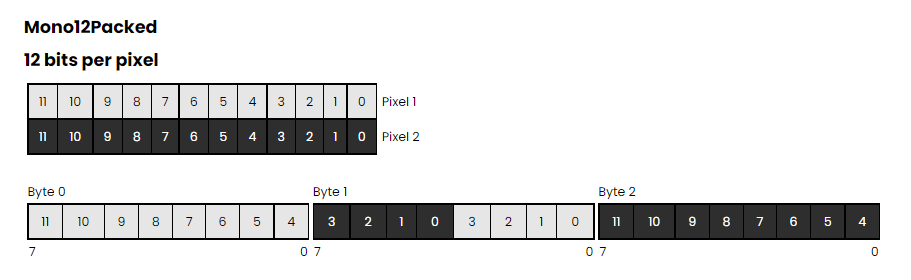
\includegraphics[width=\textwidth]{figures/Mono12Packed.png}
    \caption{Bit layout of the \cite{fisherRe15406LUT2023}}
    \label{fig:mono12packed}
\end{figure}

\begin{listing}[H]
    \begin{minted}{cuda}
        template <int width, int width_in>
        __device__ __forceinline__ void unpack10(__half2 *work_row, 
                                                 const unsigned int *img_row,
                                                 int tx) {
            __half2 *const out = &work_row[tx * 8 + 2];
        
            if (tx * 5 < width_in) {
                unsigned int buf_a, buf_b;
                buf_a = img_row[tx * 5];
                buf_b = img_row[tx * 5 + 1];
                out[0] = __halves2half2(buf_a & 0b1111111111, 
                                        buf_a >> 10 & 0b1111111111);
                out[1] = __halves2half2(buf_a >> 20 & 0b1111111111,
                                        buf_a >> 30 & 0b11 | (buf_b & 0b11111111) << 2);
        
                buf_a = img_row[tx * 5 + 2];
                out[2] = __halves2half2(buf_b >> 8 & 0b1111111111, 
                                        buf_b >> 18 & 0b1111111111);
                out[3] = __halves2half2(buf_b >> 28 & 0b1111 | (buf_a & 0b111111) << 4,
                                        buf_a >> 6 & 0b1111111111);

                buf_b = img_row[tx * 5 + 3];
                out[4] = __halves2half2(buf_a >> 16 & 0b1111111111,
                                        buf_a >> 26 & 0b111111 | (buf_b & 0b1111) << 6);
                out[5] = __halves2half2(buf_b >> 4 & 0b1111111111, 
                                        buf_b >> 14 & 0b1111111111);
        
                buf_a = img_row[tx * 5 + 4];
                out[6] = __halves2half2(buf_b >> 24 & 0b11111111 | (buf_a & 0b11) << 8,
                                        buf_a >> 2 & 0b1111111111);
                out[7] = __halves2half2(buf_a >> 12 & 0b1111111111, 
                                        buf_a >> 22 & 0b1111111111);
            }
            if (tx < 2) {
                work_row[tx] = work_row[tx + 2];
            } else if (tx >= width - 2 && tx < width) {
                work_row[tx + 4] = work_row[tx + 2];
            }
        }
    \end{minted}
    \caption{Bit unpacking in \cuda}
\end{listing}

\subsection{Debayering}
\cite{getreuerMalvarHeCutlerLinearImage2011}

\begin{listing}[H]
    \begin{minted}{python}
        class Myprinter(CXX11CodePrinter):
            def _print_Indexed(self, expr: sp.Indexed):
                return f"{expr.base}[{expr.indices[0]}][{expr.indices[1]}]"

            def _print_Float(self, expr):
                return f"__float2half2_rn({expr:.9e}f)"

            def _print_Add(self, expr: sp.Add):
                args = list(expr.args)
                toadd = []
                out = ""
                for i, el in enumerate(args):
                    if isinstance(el, sp.Float):
                        toadd.append(el)
                        continue
                    assert isinstance(el, sp.Mul) and len(el.args) == 2
                    arg0 = self._print(el.args[0] / 1024)
                    arg1 = self._print(el.args[1])
                    if i == len(args) - 1:
                        out += f"tmp =__hfma2_sat({arg0}, {arg1}, tmp);\n"
                    else:
                        out += f"tmp =__hfma2({arg0}, {arg1}, tmp);\n"
                out = f"__half2 tmp = {self._print_Float(sum(toadd))};\n" + out
                return out
        \end{minted}
    \caption{Code printer to perform multiply and add operations on \halftwo}
\end{listing}

\begin{listing}[H]
    \begin{minted}{cuda}
        __device__ __forceinline__ __half2 handle_u(__half2 **data, int col) {
            __half2 tmp = __float2half2_rn(5.000000000e-1f);
            tmp = __hfma2(__float2half2_rn(9.466415405e-5f), data[1][col + 1], tmp);
            tmp = __hfma2(__float2half2_rn(9.466415405e-5f), data[3][col - 1], tmp);
            tmp = __hfma2(__float2half2_rn(1.801812744e-4f), data[3][col + 1], tmp);
            tmp = __hfma2(__float2half2_rn(9.701843262e-6f), data[2][col + 3], tmp);
            tmp = __hfma2(__float2half2_rn(9.701843262e-6f), data[5][col], tmp);
            tmp = __hfma2(__float2half2_rn(1.483016968e-5f), data[3][col + 3], tmp);
            tmp = __hfma2(__float2half2_rn(1.483016968e-5f), data[5][col + 1], tmp);
            tmp = __hfma2(__float2half2_rn(2.661132812e-5f), data[1][col - 1], tmp);
            tmp = __hfma2(__float2half2_rn(-4.560012817e-5f), data[3][col + 2], tmp);
            tmp = __hfma2(__float2half2_rn(-4.560012817e-5f), data[4][col + 1], tmp);
            tmp = __hfma2(__float2half2_rn(-2.799591064e-5f), data[2][col + 2], tmp);
            tmp = __hfma2(__float2half2_rn(-2.799591064e-5f), data[4][col], tmp);
            tmp = __hfma2(__float2half2_rn(-1.025665283e-5f), data[1][col + 2], tmp);
            tmp = __hfma2(__float2half2_rn(-1.025665283e-5f), data[4][col - 1], tmp);
            tmp = __hfma2(__float2half2_rn(-8.205322266e-5f), data[2][col + 1], tmp);
            tmp = __hfma2(__float2half2_rn(-8.205322266e-5f), data[3][col], tmp);
            tmp = __hfma2(__float2half2_rn(-6.098022461e-6f), data[4][col + 2], tmp);
            tmp = __hfma2(__float2half2_rn(-9.701843262e-6f), data[0][col], tmp);
            tmp = __hfma2(__float2half2_rn(-9.701843262e-6f), data[2][col - 2], tmp);
            tmp = __hfma2(__float2half2_rn(-1.483016968e-5f), data[0][col + 1], tmp);
            tmp = __hfma2(__float2half2_rn(-1.483016968e-5f), data[3][col - 2], tmp);
            tmp = __hfma2(__float2half2_rn(-1.607482910e-5f), data[2][col], tmp);
            tmp = __hfma2(__float2half2_rn(-2.106811523e-5f), data[1][col], tmp);
            tmp = __hfma2_sat(__float2half2_rn(-2.106811523e-5f), data[2][col - 1], tmp);
            return __hfma2(__float2half2_rn(1023.0f), tmp, __float2half2_rn(0.0f));
        }
      \end{minted}
    \caption{Generated function}
\end{listing}

\subsubsection{Issue with max value}
\subsection{Color space conversion}

\subsection{Packagig}